\section{THEORIE}
% Edit below
\subsection{De lensvergelijking}
    %\begin{align}
    %x \times x   &= (x \times x) + 0  &&\textit{ Neutr. El. }+\\
    %        &= (x \times x) + (x \times \neg x) && \textit{ %Compl. }\times \\
    %        &= x + (x \times \neg x) && \textit{ Distr. }+ \\
    %        &= x + 0 && \textit{ Compl. }\times\\
    %        &= x && \textit{ Neutr. El. }+
    %\end{align}
De werking van de lens kan benaderd worden als een geometrisch probleem in twee dimensies. De voorstelling van de werking van de lens is te zien in \cref{fig:lensvgl}
\begin{figure}[H]
    \centering
    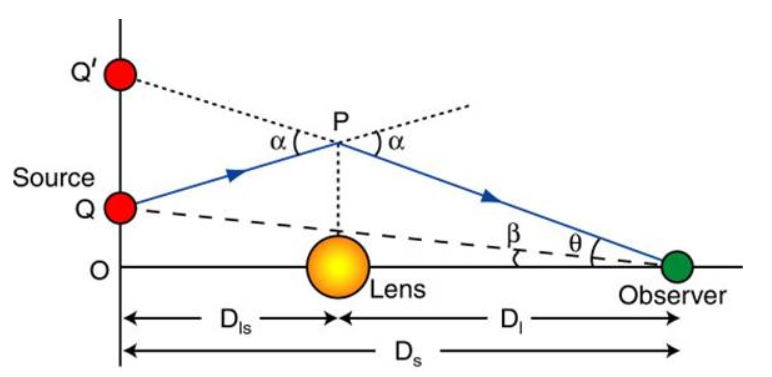
\includegraphics[scale=0.5]{Figures/Lensvergelijking.png}
    \caption{Schets van de werking van de lens in twee dimensies.}
    \label{fig:lensvgl}
\end{figure}\mbox{}
Om de lensvergelijking af te leiden wordt er gezocht naar de afstanden $OQ$, $OQ'$ en $QQ'$. Er wordt steeds aangenomen dat de hoeken klein zijn. Uit de figuur volgt er dat
$$tan(\beta) = \frac{|OQ|}{D_{s}}$$
$$|OQ| = D_{s}tan(\beta)$$
Doordat de hoeken klein zijn kunnen we Taylor rond $\beta=0$ toepassen. Er word dan gevonden dat
\begin{equation}
  |OQ| = D_{s}\beta  
  \label{for:OQ}
\end{equation}
Analoog voor $|OQ'|$ geldt er
\begin{equation}
   |OQ'| = D_{s}\theta 
   \label{for:OQ'}
\end{equation}
Om de afstand $|QQ'|$ te bepalen wordt er gewerkt in de driehoek $\Delta PQQ'$. Een close-up van de driehoek is te zien in \cref{fig:driehoek}.
\begin{figure}[h]
    \centering
    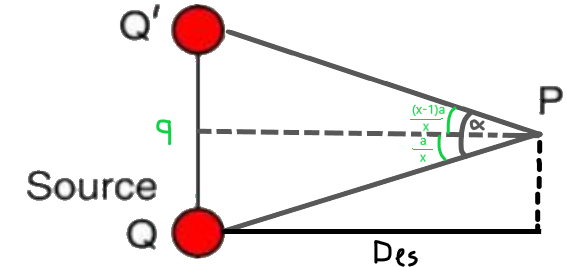
\includegraphics[scale=0.45]{Figures/driehoek.png}
    \caption{Close-up van de desbetreffende driehoek}
    \label{fig:driehoek}
\end{figure}
Er wordt opgemerkt dat $|QQ'| = |Qq|+|qQ'|$. Die twee afstanden zijn makkelijk te vinden uit de tangens. De hoek $\alpha$ wordt gesplitst in twee hoeken (die optellen tot $\alpha$). Zo wordt een rechthoekige driehoek verkregen. De eerste hoek is dan $\frac{\alpha}{x}$. De tweede hoek is gegeven door $\frac{(x-1)\alpha}{x}$. Zo zijn de twee afstanden gegeven door
$$tan(\frac{\alpha}{x})=\frac{|Qq|}{D_{ls}}$$
$$|Qq|=tan(\frac{\alpha}{x})D_{ls}$$
Analoog wordt er gevonden
$$tan(\frac{(x-1)\alpha}{x})=\frac{|qQ'|}{D_{ls}}$$
$$|qQ'|=tan(\frac{(x-1)\alpha}{x})D_{ls}$$
De som is dan gegeven door
$$|QQ'|=D_{ls}(tan(\frac{\alpha}{x})+tan(\frac{(x-1)\alpha}{x}))$$
Doordat de hoek $\alpha$ klein is kan er Taylor toegepast worden op de tangens, rond 0. Dan wordt er gevonden dat
\begin{align}
    |QQ'| &=D_{ls}(\frac{\alpha}{x}+\frac{x\alpha}{x}-\frac{\alpha}{x}) \nonumber\\
    &=D_{ls}\alpha
    \label{for:QQ'}
\end{align}
Nu de afstanden $|OQ|, |OQ'|$ en $|QQ'|$ gekend zijn (zie \cref{for:OQ}, \cref{for:OQ'} en \cref{for:QQ'}), kan de lensvergelijking gevonden worden. Het is eenvoudig in te zien dat $|OQ'|=|OQ|+|QQ'|$. Daaruit volgt
\begin{align}
    D_{s}\theta &=D_{s}\beta + D_{ls}\alpha \nonumber\\
    \theta &= \beta + \frac{D_{ls}}{D_{s}}\alpha \nonumber\\
    \beta &= \theta - \frac{D_{ls}}{D_{s}}\alpha
    \label{for: lensvgl}
\end{align}
\cref{for: lensvgl} wordt de lensvergelijking genoemd.
\subsection{Newtoniaanse bepaling afbuighoek als gevolg van een gravitationeel veld}
Er wordt vertrokken vanuit de bewegingsvergelijkingen voor een deeltje in een potentiaal, gecreëerd door het zwaartekrachtveld. Er wordt aangetoond dat de oplossingen van de bewegingsvergelijking kegelsneden (cikel, ellips, hyperbool, parabool) als oplossing heeft.
\subsubsection{De baan van een deeltje in een zwaartekrachtveld zijn kegelsneden}
Voor gravitatie wordt de potentiële energie gegeven door
$$V(r)=-\frac{GmM}{r}$$
De effectieve potentiële energie is gegeven door
$$V_{eff}(r)=-\frac{k}{r}+\frac{l^{2}}{2\mu r^{2}}$$
Hierin is $k=GmM$.\\
De bewegingsvergelijking wordt dan gegeven door
$$\mu\ddot{r}=\frac{l^{2}}{\mu r^{3}}-\frac{k}{r^{2}}$$
Deze vergelijking is niet lineair. We voeren een nieuwe variabele in. Stel $u=\frac{1}{r}$ en $t=\phi$. We weten al dat
$$\mu r^{2}\dot{\phi}=l;\ \ \ \ \ \mu r^{2}d\phi=ldt;\ \ \ \ \ dt=\frac{\mu}{lu^{2}}d\phi$$
Dan geldt er dat
\begin{align}
\dot{r}&=\frac{d}{dt}r=\frac{d}{dt}(\frac{1}{u}) \nonumber \\
&=-\frac{1}{u^{2}}\frac{du}{dt} \nonumber \\
&=-\frac{1}{u^{2}}\frac{du}{d\phi}\frac{d\phi}{dt} \nonumber \\
&=-\frac{1}{u{2}}\frac{lu^{2}}{\mu}\frac{du}{d\phi} \nonumber \\
&=-\frac{l}{\mu}\frac{du}{d\phi} \nonumber 
\end{align}
De 2de afgeleide is gegeven door
\begin{align}
\ddot{r}&=\frac{d}{dt}[-\frac{l}{\mu}\frac{du}{dt}] \nonumber \\
&=-\frac{l}{\mu}\frac{d}{d\phi}(\frac{du}{d\phi})\frac{d\phi}{dt} \nonumber \\
&=-\frac{l}{\mu}\frac{lu^{2}}{\mu}\frac{d^{2}u}{d\phi^{2}} \nonumber 
\end{align}
Dan krijgen we als differentiaalvergelijking van de baan dat
$$\frac{d^{2}u}{d\phi^{2}}+u=\frac{k\mu}{l^{2}}$$
De oplossing van deze differentiaalvergelijking is gegeven door
$$u(\phi)=\frac{\mu k}{l^{2}}+Acos(\phi)$$
We gaan nu overgaan op Cartesische coördinaten. Stel $p=\frac{l^{2}}{\mu k}$ en stel $\epsilon=pA\geq0$. Dan geldt er
$$pu=1+\epsilon cos(\phi)$$
$$p=r+r\epsilon cos(\phi)$$
$$(p-\epsilon x)^{2}=x^{2}+y^{2}$$
De energie is gegeven door
$$E=\frac{1}{2}\mu(\dot{r}^{2}+r^{2}\dot{\phi}^{2})-\frac{k}{r}$$
$$=\frac{\mu k^{2}}{2l^{2}}(\epsilon^{2}-1)$$
Merk op dat de energie afhankelijk is van $\epsilon$. 
\begin{itemize}
\item  $\epsilon=0$: we hebben een minimum van de energie. Er geldt
$$x^{2}+y^{2}=p^{2}$$
Dit is exact gelijk aan de vergelijking van een cirkel met als straal p. Deze straal is exact gelijk aan het minimum van $V_{eff}$. 
\item $\epsilon=1$, dan is de energie gelijk aan 0. De baan is dan gegeven door
$$p{2}+x^{2}-2px=x^{2}+y^{2}$$
$$2px=p^{2}-y^{2}$$
$$x(y)=\frac{p^{2}-y^{2}}{2p}$$
Dit is de baan van een parapbool
\item $0<\epsilon<1$, dit komt overeen met een energie die kleiner is dan 0. De baan is dan gegeven door
$$p^{2}+\epsilon^{2}x^{2}-2\epsilon px-x^{2}-y^{2}=0$$
$$(1-\epsilon^{2})x^{2}+2\epsilon px+y^{2}-p^{2}=0$$
$$(1-\epsilon^{2})(x^{2}+\frac{2\epsilon px}{(1-\epsilon^{2})}+\frac{\epsilon^{2}p^{2}}{(1-\epsilon^{2})^{2}}-\frac{\epsilon^{2}p^{2}}{(1-\epsilon^{2})^{2}})+y^{2}-p^{2}=0$$
$$(1-\epsilon^{2}))(x+\frac{\epsilon p}{(1-\epsilon^{2})})^{2}+y^{2}-\frac{\epsilon^{2}p^{2}}{(1-\epsilon^{2})}-p^{2}=0$$
$$(1-\epsilon^{2})(x+\frac{\epsilon p}{(1-\epsilon^{2})})^{2}+y^{2}=\frac{p^{2}}{(1-\epsilon^{2})}$$
Dit kunnen we ook nog schrijven als
$$\frac{(x-x_{c})^{2}}{a^{2}}+\frac{y^{2}}{b^{2}}=1$$
Met: \\
$x_{c}=\frac{-\epsilon p}{1-\epsilon^{2}}$ \\
$p=\frac{l^{2}}{\mu k}$\\
$\epsilon = pA$\\
$a=\frac{p}{1-\epsilon^{2}}$\\
$b=\frac{p}{\sqrt{1-\epsilon^{2}}}$\\
Dit komt overeen met de baan van een ellips
\item $\epsilon > 0$, dit komt overeen met een energie die groter is dan 0. 
$$\frac{(x-x_{c})^{2}}{a^{2}}-\frac{y^{2}}{b^{2}}=1$$
Dit is de baan van een hyperbool
\end{itemize}
\subsubsection{De bijhorende afbuighoek voor een hyperbolische baan}
De kinetische energie van het deeltje in de potentiaal (per eenheidsmassa) is gegeven door 
\begin{equation}
    E=\frac{1}{2}mv^{2}
    \label{for:energie}
\end{equation}
Het draaimoment per eenheidsmassa is gegeven door
\begin{equation}
    L=rv
    \label{for:draaimoment}
\end{equation}
Deze twee grootheden kunnen ook geschreven worden in termen van de lange en korte as van de kegelsneden:
\begin{equation}
    E = \frac{GM}{2a}
    \label{for:E}
\end{equation}
\begin{equation}
    L^2 = \frac{GMb^{2}}{a}
    \label{for:L2}
\end{equation}
De halve hoek van de hyperbolische baan is dan gegeven door 
\begin{equation}
    tan(\beta) = \frac{b}{a}
    \label{for: hoek}
\end{equation}
We gaan \cref{for: hoek} herschrijven in termen van L (\cref{for:L2}) en E (\cref{for:E}).
Merk op dat
$$E\cdot L^{2}=\frac{G^{2}M^{2}b^{2}}{2a^{2}}$$
$$\frac{2E\cdot L^{2}}{G^{2}M^{2}}=\frac{b^{2}}{a^{2}}$$
$$\frac{\sqrt{2E}L}{GM}=\frac{b}{a}$$
Invullen van \cref{for:energie} en \cref{for:draaimoment} geeft
\begin{align}
    \frac{b}{a}&=\frac{\sqrt{2\cdot\frac{1}{2}v^{2}}rv}{GM} \nonumber \\
    &= \frac{rv^{2}}{GM} \nonumber \\
    tan(\beta) &=\frac{rv^{2}}{GM} 
    \label{for:tangens}
\end{align}
Voor de afbuighoek geldt er dan:
$$\theta = \pi - 2\beta$$
Omvormen naar $\beta$ geeft
$$\beta = \frac{\pi}{2}-\frac{\theta}{2}$$
De tangens nemen
\begin{equation}
    tan(\beta) = tan(\frac{\pi}{2}-\frac{\theta}{2})
    \label{for:tan}
\end{equation}
We herschrijven de laatste tangens:
\begin{align}
    tan(\frac{\pi}{2}-\frac{\theta}{2})&=\frac{sin(\frac{\pi}{2}-\frac{\theta}{2})}{cos(\frac{\pi}{2}-\frac{\theta}{2})}\nonumber\\
    &= \frac{cos(\frac{\theta}{2}}{sin(\frac{\theta}{2}}\nonumber \\
    & = cot(\frac{\theta}{2})
    \label{for:cot}
\end{align}
Invullen van \cref{for:cot} in \cref{for:tan} geeft
\begin{equation}
    tan(\beta) = \frac{1}{tan(\frac{\beta}{2})}
    \label{for:afbuighoek}
\end{equation}
Invullen van \cref{for:tangens} en Taylor toepassen voor kleine $\theta$
$$\frac{1}{tan(\frac{\theta}{2})} = \frac{rv^{2}}{GM}$$
$$\frac{1}{\frac{\theta}{2}}=\frac{rv^{2}}{GM}$$
$$\frac{\theta}{2} = \frac{GM}{rv^{2}}$$
$$\theta = \frac{2GM}{rv^{2}}$$
Als de afbuiging van licht beschouwd wordt is de snelheid gegeven door de snelheid van het licht. Dan is de afbuighoek gegeven door \cref{for: afbuighoek}.
\begin{equation}
    \theta = \frac{2GM}{rc^{2}}
    \label{for: afbuighoek}
\end{equation}
Dit was nu de afleiding voor de hyperbool. 
\\ ???? KAN DAT ???? \\
Als het foton geen hyperbolische baan volgt, dan komt het vast te zitten. Uit de 2de wet van Kepler volgt ook dat gelijke oppervlakke in gelijke tijd beschreven worden. Daaruit volgt dan dat de snelheid van het deeltje afhankelijk is van de kromming van de baan. En dat is een probleem, want onze snelheid is de lichtsnelheid, en die kan nie groter worden. Een hyperbolische baan (of parabolisch, dat is gewoon een speciaal geval van de hyperbool) is dus de enige optie.
Analoog kan hetzelfde gedaan worden voor de ellips en parabool. Het enige dat verandert is de energie.\\
Voor de elllips geldt:
$$E=-\frac{GM}{2a}$$
Voor de parabool geldt:
$$E=0$$


